%%%%%%
% Metadata
%%%%%%
\chapter{Conclusion and Future Directions}
\label{chapter:Conclusion}
\section{Summary of the Study}


This thesis addressed the problem of using a fixed significance level, commonly $\alpha = 0.05$, in hypothesis testing. Although widely used, this threshold is often applied without considering the specific characteristics of a study\cite{CowlesDavis1982}. Such uniform use may contribute to misleading statistical decisions and replication failures\cite{Benjamin2018}\cite{WassersteinLazar2016}.

To address this issue, a 
 alpha recommendation system was developed. The system uses replication data to learn patterns between sample size, effect size, and study outcomes. A Random Forest regression model was trained to estimate a $\alpha_{base}$ value based on these study characteristics. In addition to this data driven component, contextual adjustments were incorporated to account for user preferences such as risk tolerance, test direction, and multiple hypothesis testing.

The system was implemented in Python and deployed through a Streamlit interface, allowing users to input study information and receive a recommended significance level in a structured and accessible manner.

\section{Main Findings}


The main finding is that the system recommended a significance 
level stricter than $0.05$ in 13 out of 20 cases where the 
conventional threshold had led to a false positive decision, 
suggesting that a data driven approach can support more cautious 
and reproducible statistical conclusions.

\begin{figure}[H]
	\centering
	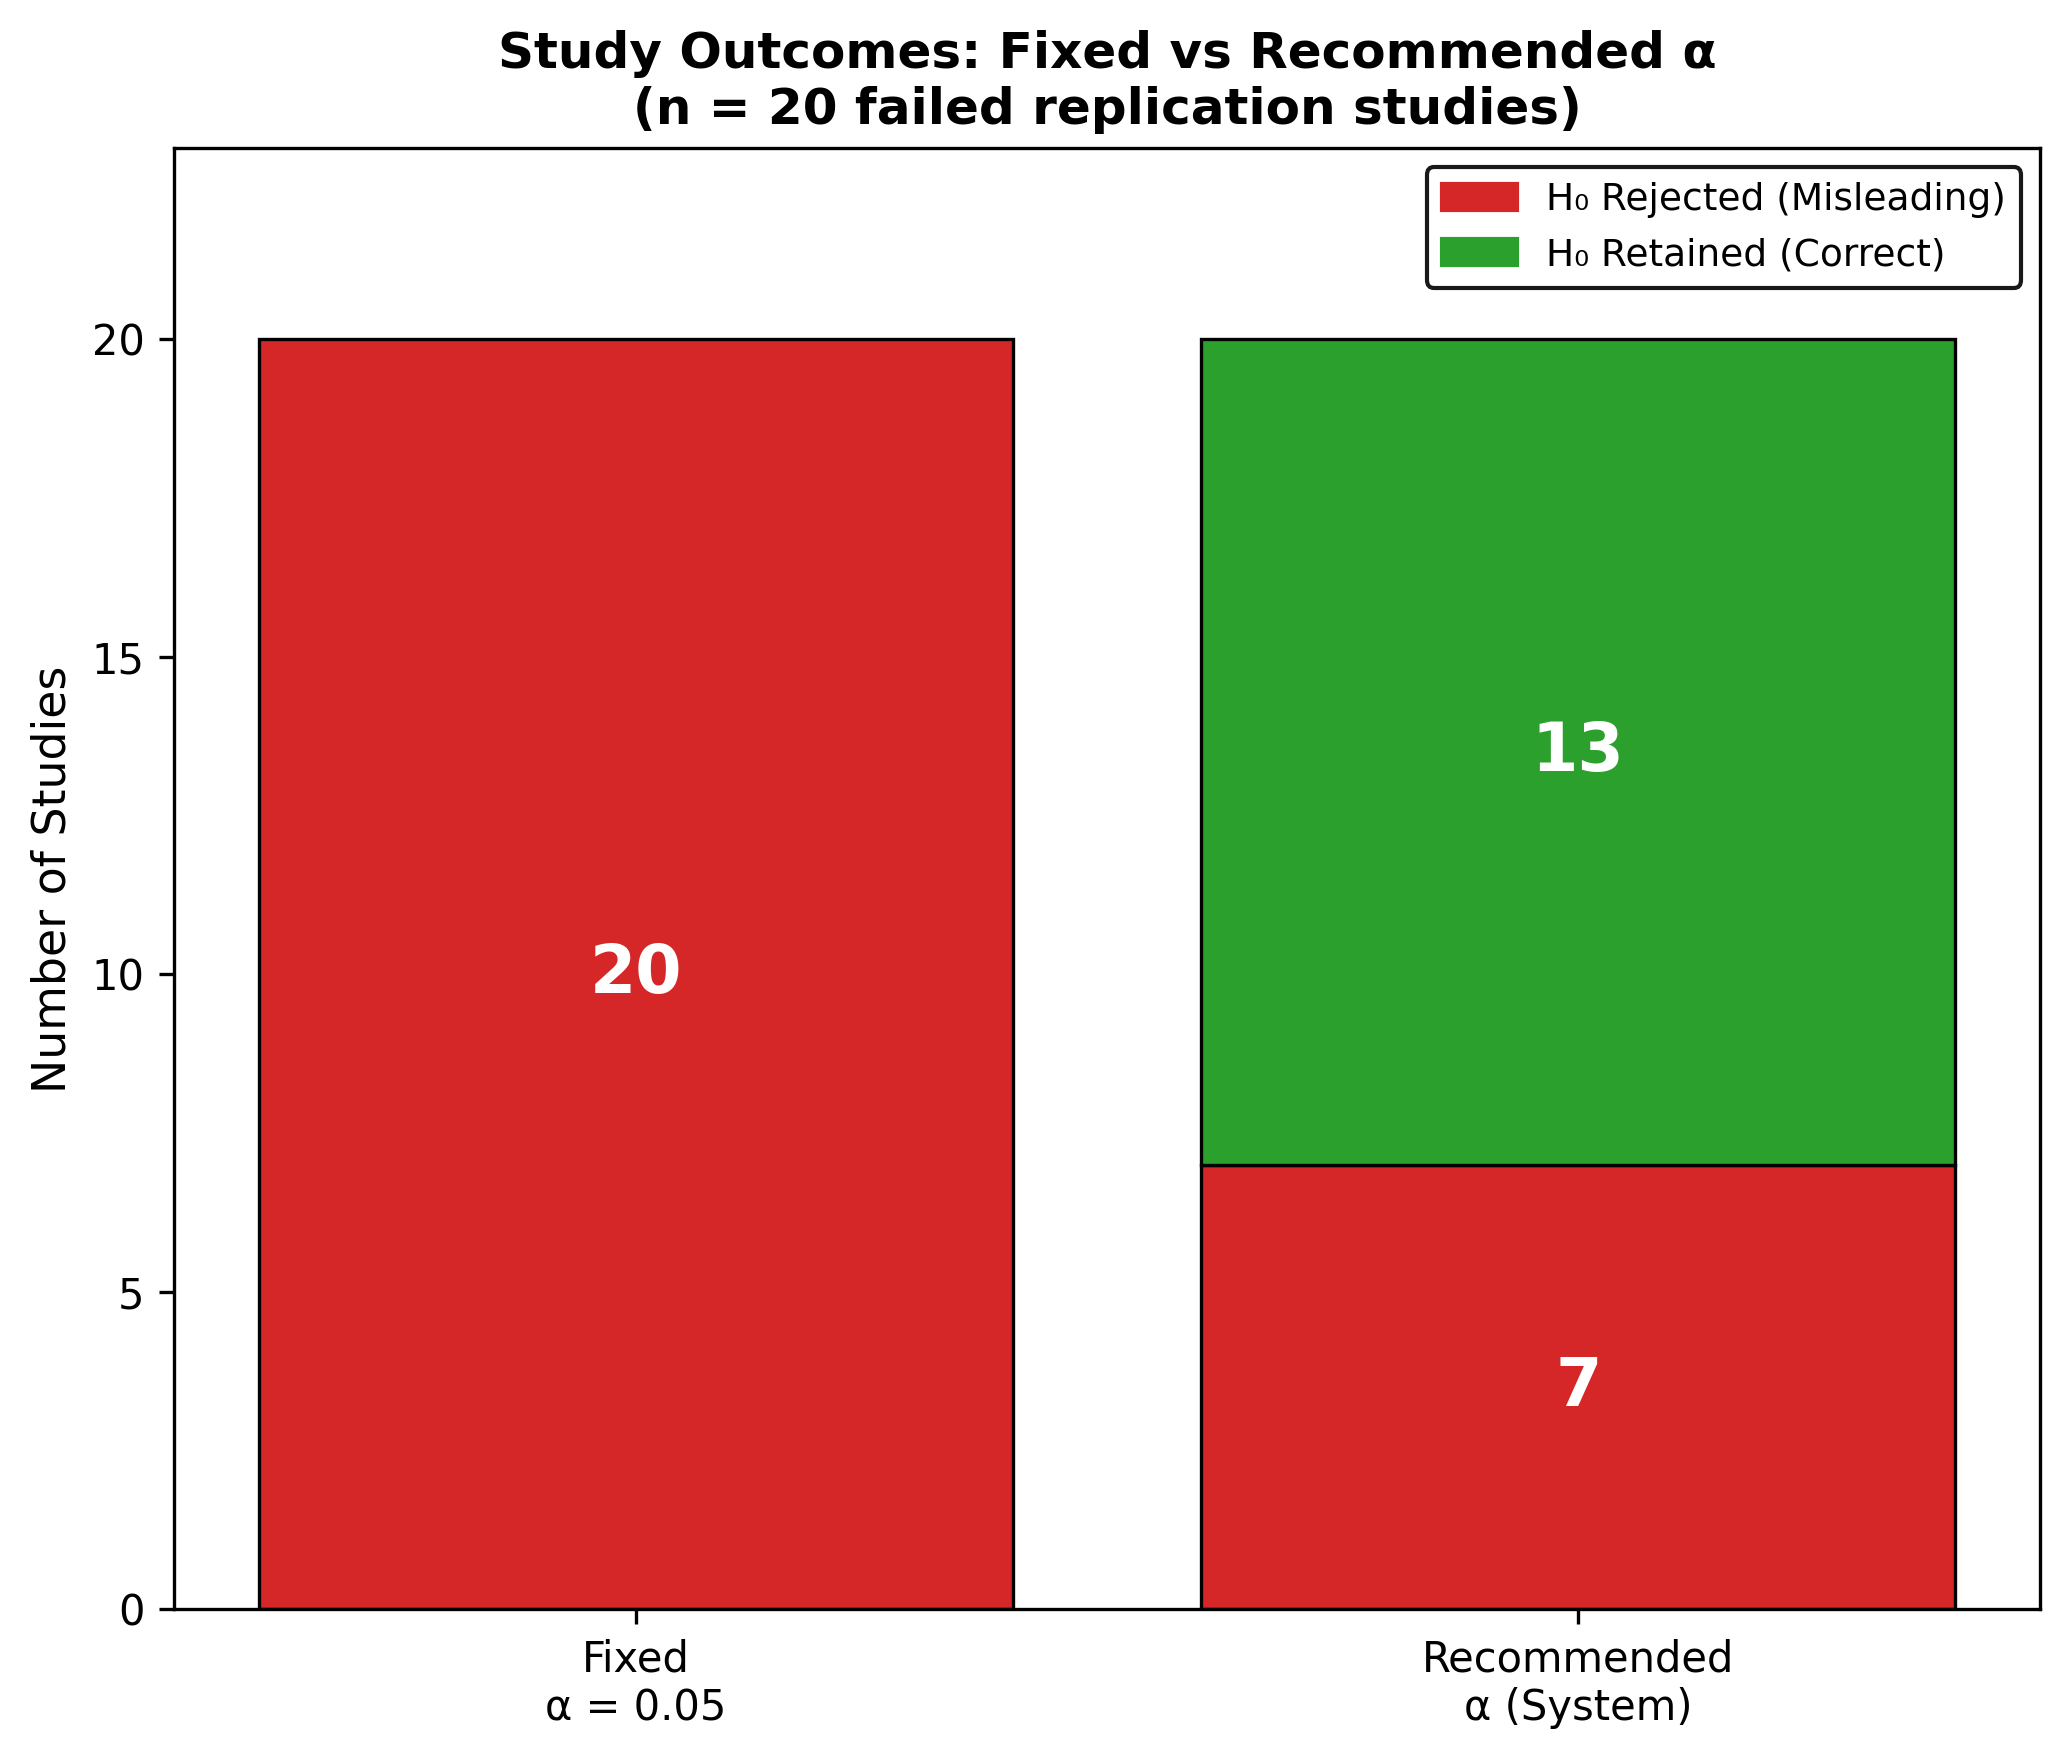
\includegraphics[width=0.7\textwidth]{Images/study_outcomes_chart}
	\caption{Comparison of study outcomes}
	\label{fig:Comparision}
\end{figure}
Overall, the findings support the idea that the significance level should not be treated as a universal constant but instead should reflect both empirical patterns from prior research and the specific context of each study.

\section{Limitations}
Several limitations of this study should be noted.

First, the evaluation was conducted using 20 failed replication studies from different research fields. Although these studies provide useful examples, a larger number of studies would allow a broader evaluation of the system.

Second, the contextual adjustment factors used in the system were implemented using heuristic scaling rules. These adjustments were inspired by ideas from decision theory\cite{Berger1985}, but the exact numerical values were chosen for simplicity and interpretability.

Third, neutral contextual settings were used during the evaluation. This decision was made because the original studies did not report the researchers’ preferences, such as their risk tolerance or testing strategy. Using neutral settings allowed the studies to be compared under the same conditions, but it does not fully capture how different researcher preferences might influence the recommended alpha values.

Fourth, the proposed system does not determine sample size and does not replace traditional power analysis. It assumes that important study parameters, such as sample size and expected effect size, are already specified by the researcher. Additionally, while the system can in principle be applied across common hypothesis tests including t-tests, chi-squared tests, and F-tests, since sample size and effect size can be derived from all of these it does not guide the researcher in selecting which test to use. The system focuses solely on recommending a suitable significance threshold, assuming the appropriate test type has already been chosen.

Overall, these limitations indicate that the proposed system should be viewed as a decision support tool that complements existing statistical practices rather than replacing established methods of study design and statistical inference.

\section{Future Research Directions}

Future research can extend the proposed system in several directions.

First, the contextual scaling factors used in this study could be further increased using formal decision theoretic models. Developing such models would require a deeper theoretical analysis and empirical calibration across many studies, which is beyond the scope of the present work.

Second, the machine learning model could be trained on a larger and more diverse collection of replication datasets from additional scientific disciplines. Expanding the dataset would allow the system to learn broader statistical patterns and improve the generalizability of the alpha recommendations.

Third, future studies could compare the proposed approach with alternative statistical frameworks, such as Bayesian methods \cite{Berger1985} or adaptive error control procedures\cite{Benjamini1995}. Such comparisons would help evaluate how the proposed system performs relative to other approaches for managing statistical uncertainty.

Fourth, the system could be extended to integrate power analysis. This would allow the framework to provide guidance not only on the choice of significance level but also on appropriate sample size during study design.

Finally, future work could explore the development of field specific models that account for differences in research practices and replicability patterns across disciplines. This could help tailor alpha recommendations to the methodological characteristics of particular scientific fields.

\section{Final Remarks}

This thesis demonstrates that significance level selection can be approached as a data informed and context sensitive decision rather than as a fixed convention. By combining replication evidence with user defined preferences, the proposed alpha recommendation system provides a structured framework for more flexible statistical decision making.

While further refinement is possible, the study contributes to the ongoing discussion on improving research reliability and encourages a more thoughtful approach to hypothesis testing across disciplines.
